\begin{figure*}[htbp]
\begin{center}
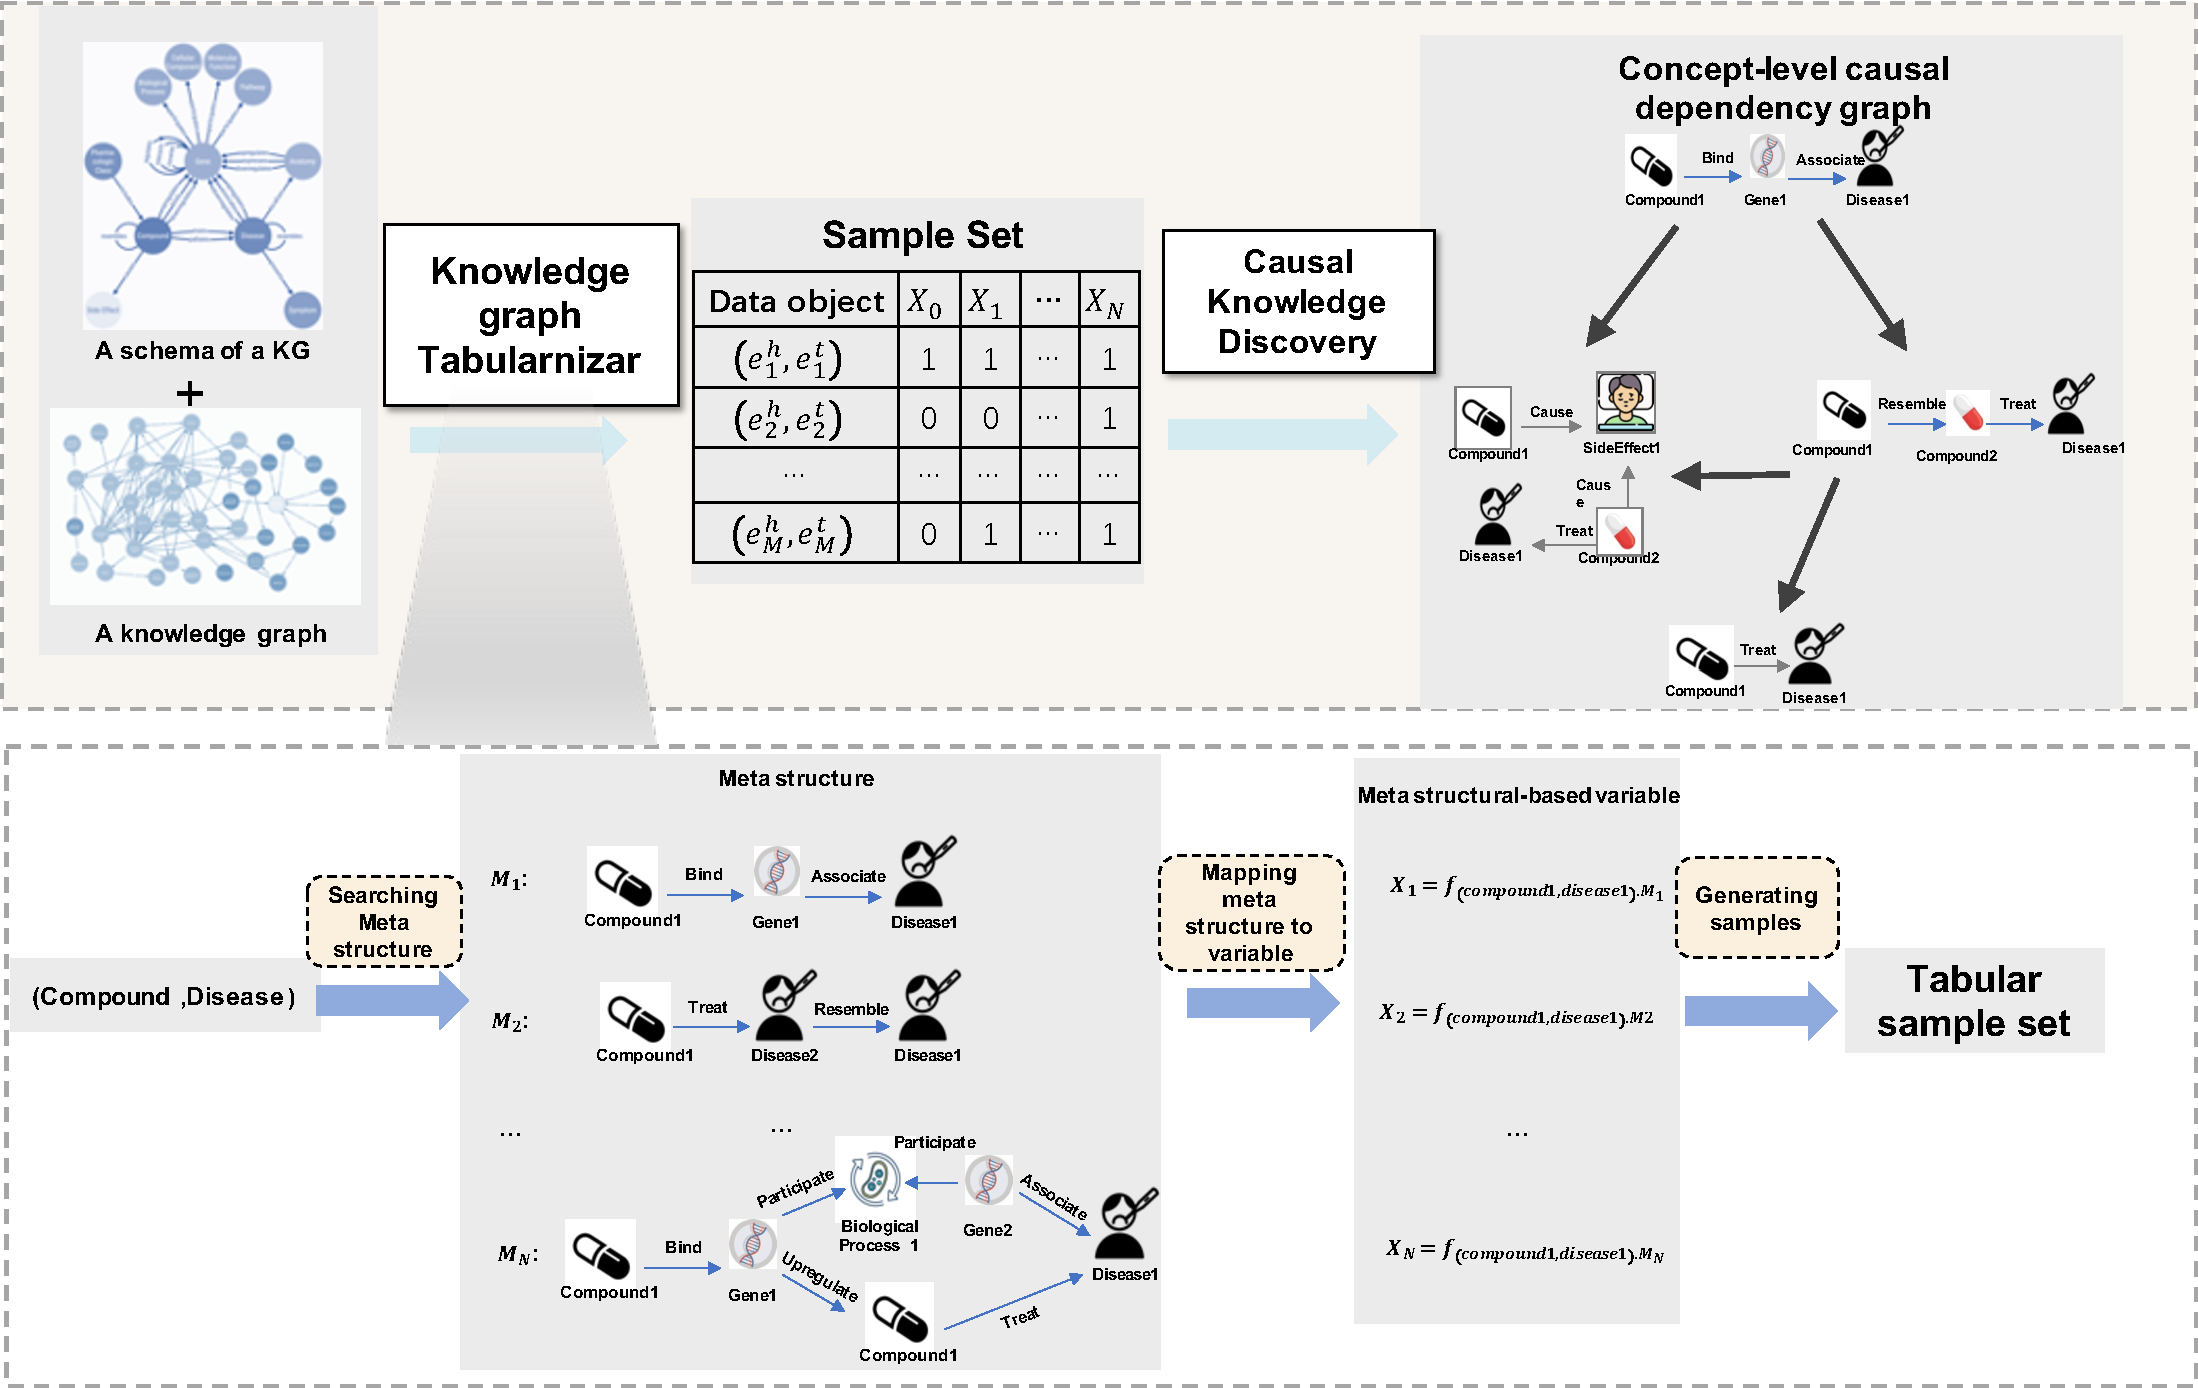
\includegraphics[width=18cm]{submissions/causal-meta-knowledge/figures/framework.pdf}
\end{center}
\caption{The architecture of~\dname}
\label{fig:framwork}
\end{figure*}
In the last section, we introduce the SPRM, which is a Bayesian model defined on the meta structural variables.
In this section, we will presents the practical method to learn the SPRM $\Pi$ from a given KG.
Especially, we focus on the learning of the structure $\mathcal{S}$.
Because structure $\mathcal{S}$ is the fundamental of parameter $\mathcal{S}$ in SPRM, and the exploration of model parameters demands assumptions on the probability distribution followed by the data, hence limiting the applicability of the model.
In the next section, we will show the structural information is already available for downstream tasks such as link prediction.
The architecture of the structure learning method is shown in Fig~\ref{fig:framwork}.


\subsection{Knowledge Graph Tabularnizar}
% \begin{wrapfigure}{r}{0.2\texotwidth}
% 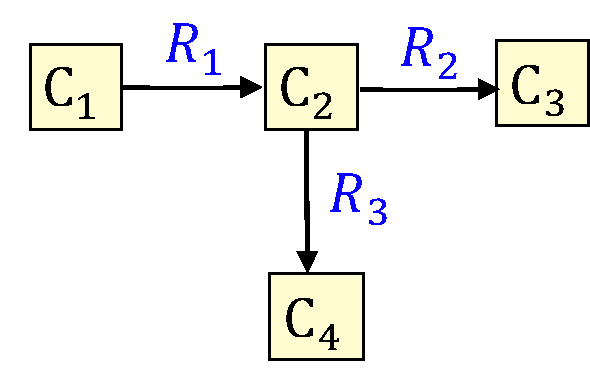
\includegraphics[width=0.2\textwidth]{./fig/path_examplev2.pdf}
% \caption{An illustrative KGS, which includes four concepts and three relations.}
% \label{fig:path_example}
% \end{wrapfigure}


The traditional causal discovery algorithm aims to learn the whole causal structure, without any prior knowledge about the skeleton of the structure or the orientation of the causal relationship.
% which includes all causal relationships between the involved variable.
% The causal structure can be represented as a DAG, where each node indicates an involved variable.
% Discovering causal relationships from observational data
% by a set of causal relationships among a set of variables, and the causal discovery is normally regarded as a the problem of learning the \textit{whole} causal structure from observational data in the prior works.
However, the fundamental tasks in KG, such as KG completion and KG reasoning, mainly concern the single relation.
Therefore, the main goal of rule mining is to find the body structure for a given head relation.
Consequently, in this paper, we only need to solve a \textit{local} causal discovery problem, which is to find all the direct causes for a given KGS-based variable.
Here we propose an efficient causal rule discovery method, \textit{\dname}, which performs the following steps:

\noindent
\textbf{Step-1: Data-Driven Path Finding}.
According to assumption~\ref{ass:candidata}, any KGS, which can support any entity pair $(e^h \in \mathcal{E}^h, e^t \in \mathcal{E}^t)$, is a valid candidate cause for $S^{E}(v^{h,E},v^{t,E})$, where $E^h$ and $E^t$ are the entity set corresponding to $C^h,C^t$ in KG $\mathcal{G}$, respectively.
So we find all the candidate causes by searching all the paths between entity pairs $(e^h, e^t)$, which renders variable $S^{E}(v^{h,E},v^{t,E})$ as true, based on the following considerations:
\begin{itemize}
\item[1)] Any graph contains two specific nodes can be represented as a path between them (duplicate nodes are permitted).
For example, as shown in Fig.\ref{fig:path_example}, the structure between $C_1$ and $C_2$ can be determined by the path $C_1 \stackrel{R_1}{\longrightarrow} C_2 \stackrel{R_3}{\longrightarrow} C_4 \stackrel{R_3}{\longleftarrow} C_2 \stackrel{R_2}{\longrightarrow} C_3$.

\item[2)]  There are many well-studied path finding algorithms, which can search the paths under different types of constraints, such as Dijkstra’s algorithm~\cite{lanning2014dijkstra}, A* search~\cite{cui2011based}, best-first search~\cite{heusner2018best}, etc.
These off-the-shelf methods can be directly adopted to our framework.
In the experiments, we adopt the best-first search algorithm.

\item[3)] Lots of existing rule mining methods~\cite{sadeghian2019drum,yang2017differentiable,ho2018rule} designed for the \textit{closed rules}, meaning that each entity set appears in at least two edges of the rule.
It renders the path-like graph structure in most cases.
\end{itemize}
\vspace{-2pt}
Since the number of candidate KGS can be the power level of the number of relation types, we require that any KGS created during path finding need to be supported by at least $a_{sup}$ entity pair $(e^h,e^t)$ in the training KG, and the length of the path is no more than $\ell$, where $a_{sup}$ and $\ell$ are the hyper-parameters.

\noindent
\textbf{Step-2: Refinement of the Identical Relations}.
In KG, there may be some identical relations, even though they have different relation names.
For example, Wife(A,B) $\leftrightarrow$ Husband(B,A), if A is the wife of B, then B must be the husband of A.
However, they will lead the invalid independence test in the following causal discovery step, even though these two relations have very strong causal relationship with each other.
In particular, based on the causal variable and sample definitions in KG (Sec.~\ref{sec:v_a_s}), these two relations are the same variables for the causal discovery method, since the values of their samples are the same all the time.
When one relation is treated as the conditional variable in the independent test of the other one, the conditional independence (CI) test $CI(X,Y|X)$ will be judged as independent.
So for an analyzed KGS $S_E$, we search all the identical KGSs in the input KG and temporarily remove them from the candidate cause set in the independent test period.
The causal rules which include the identical KGSs will have the highest weight, when they are applied into the downstream tasks.

\noindent
\textbf{Step-3: PC-like Causal Rule Discovery}.
PC algorithm~\cite{tsagris2019bayesian} is a prototypical constraint-based algorithm for learning-based Bayesian networks.
This algorithm starts with the fully connected network and uses the CI test to decide whether an edge will be removed or retained.
This feature makes the PC algorithm efficient in the sparse graphs.


In our problem, we assume the causal relationships between the KGSs are sparse and propose a PC-like causal rule discovery method (Algo.~\ref{alg:pc-like}) in KG.
Particularly, given a KGS $S^{E}$~(denoted as variable $Y$ in this algorithm), for each candidate cause in $\mathcal{X}^{Ca}$~(denoted as variable $X_j$),
the proposed algorithm decides whether $X_j$ should be retained in candidate causes set $\mathcal{X}^{Ca}$ by testing the independence of $X_j$ and $Y$ conditioning on a subset $\mathcal{Z}$ of $\mathcal{X}^{Ca}\backslash \{X_j\}$.
The CI tests are organised by levels (based on the size $d$ of the conditioning sets).
At the first level ($d = 0$), all pairs of variables are tested conditioning on the empty set.
Some of the candidate causes would be removed and the algorithm only tests the remaining candidate causes in the next level ($d = 1$).
The size of the conditioning set, $d$, is progressively increased (by one) at each new level until $d$ is greater than $|\mathcal{S}^{Ca}|-1$.



\begin{algorithm}
\caption{PC-like Causal Rule Discovery}
\label{alg:pc-like}
\KwIn{$Y$ and $\{y_i\}, i=1,\dots,N$ : variable and samples of analyzed KGS $S^E$ ;
 $\mathcal{X}^{Ca} = \{X_j\}, j=1,\dots,M$ and $\{\{x_i\}_j\}, i=1,\dots,N$: variables and samples of candidate causes; }
% \KwData{$\mathcal{B}=\left\{b_{1}, \ldots, b_{n}\right\}$, $\mathcal{S}=\left\{s_{1}, \ldots, s_{n}\right\}$, $\Omega$ \\ $\mathcal{B}$ is the list of initial bounding boxes,  $\mathcal{S}$ contains corresponding scores, $\Omega$ is the NMS threshold}
\KwOut{causes $\mathcal{X}^{C}$ of $Y$}

level $d \gets 0$\;
\While{$d<= |\mathcal{X}^{Ca}|-1$}{

\For{each $X_j \in  \mathcal{X}^{Ca}$}{
    \For{each subset $\mathcal{Z} \in \mathcal{X}^{Ca} \backslash \{ X_j\}$ and $|\mathcal{Z}|=d$}{
    Test CI($X_j,Y|\mathcal{Z}$)\;
    \If{CI($X_j,Y|\mathcal{Z}$)}{
        Test CI($\mathcal{Z},Y|X_j$) \Comment{Reverse CI test.} \;
        \If{not CI($\mathcal{Z},Y|X_j$)}{
            Remove $X_j$ from $\mathcal{X}^{Ca}$\;
            Break\;
        }
    }
}
}
$d \gets d+1$\;
}
$\mathcal{X}^{C} = \mathcal{X}^{Ca}$
\vspace{-3pt}
\end{algorithm}

% \begin{algorithm}
% \caption{PC-like Causal Rule Discovery}
% \label{alg:pc-like}
% \begin{algorithmic}
% \KwIn{
% $Y$ and $\{y_i\}, i=1,\dots,N$ : variable and samples of analyzed KGS $S^E$ ;\\
% $\mathcal{S}^{Ca} = \{X_j\}, j=1,\dots,M$ and $\{\{x_i\}_j\}, i=1,\dots,N$: variables and samples of candidate causes; }
% \ENSURE causes $\mathcal{S}^{C}$ of $Y$
% \STATE Let level $d=0$
% \REPEAT
% \FOR{each $X_j \in  \mathcal{S}^{Ca}$}
%     \FOR{each subset $\mathcal{Z} \in \mathcal{S}^{Ca} \backslash \{ X_j\}$ and $|\mathcal{Z}|=d$}
%     \STATE Test CI($X_j,Y|\mathcal{Z}$)
%     \IF{CI($X_j,Y|\mathcal{Z}$)}
%         \STATE Test CI($\mathcal{Z},Y|X_j$) \Comment{Reverse CI test.}
%         \IF{CI($\mathcal{Z},Y|X_j$)}
%             \STATE Remove $X_j$ from $\mathcal{S}^{Ca}$
%             \STATE Break
%         \ENDIF
%     \ENDIF
%     \ENDFOR
% \ENDFOR
% \STATE $d=d+1$
% \UNTIL{$d> |\mathcal{S}^{Ca}|-1$}
% \STATE $\mathcal{S}^{C} = \mathcal{S}^{Ca}$
% \end{algorithmic}
% \end{algorithm}

For the CI test part in Algo.~\ref{alg:pc-like}, we test the independence between $X_j$ and $Y$ conditioning on each value of conditional variables $\mathcal{Z}$.
Only if $X_j$ is independent with $Y$ conditioning on each value of conditional variables $\mathcal{Z}$ except the all zero value, $X_j$ is judged to be independent with $Y$.
For the logical rules, the head relation are inferred by the positive statement of body relations.
When the conditional variables are all zero, the conditional variables have hardly any impact on the cause and effect variable, which violate the definition of confounders.
Let us take this situation as an example, when we examine the dependency between the kinship relations, Brother(A,C) and Sister(C,A) given the two-relations KGS Son(A,B),Son(C,B). Son(A,B),Son(C,B) can be seen as the direct cause of Son(A,C), since A must be the brother of C, if A and C are both the sons of B.
If A and C are not satisfied the KGS Son(A,B),Son(C,B), the relations Brother(A,C) and Sister(C,A) are dependent with each other, then Brother(A,C) and Sister(C,A) are judged as to be dependent given two-relations KGS Son(A,B),Son(C,B) according to the traditional CI test.
Therefore we omit the results of test when the conditional variables are all negative.
We adopt SCI algorithm~\cite{marx2019testing} as the independent test method in the experiments, which can works well on limited samples.

Different to the classic PC algorithm, we add the reverse CI test in Algo.~\ref{alg:pc-like} (line 7) to avoid interaction effect among multiple deterministic rules.
For example, in the phase when we discover the causes of the single relation KGS $S^E=$ Brother(A,C), the KGSs $S_1=$ Son(A,B), Son(C,B) and $S_2=$ Son(A,B), Daughter(C,B) are both valid candidate causes.
If any candidate cause KGS is true ($X_1=1$ or $X_2=1$), the effect KGS Brother(A,C) must be true ($Y=1$).
Therefore the tests $CI(X_1, Y|X_2=1)$ and $CI(X_2, Y|X_1=1)$ will be judged as true.
Both $S_1$ and $S_2$ will be removed from the candidate set $\mathcal{X}^{Ca}$, even though they can infer the effect KGS deterministically.
Consequently, we use the reverse CI test to avoid this situation.
In particular, if $X_j$ and $Y$ are judged to be independent conditioning on $\mathcal{Z}$, we will examine the independence between $\mathcal{Z}$ and $Y$ conditioning on $\mathcal{X}_j$.
When the result of the additional test is negative, $X_j$ will be removed from $\mathcal{X}^{Ca}$. 